\section{Use-Case}
\label{sect:useCase}

To demonstrate the cit-storm framework a twitter stream is analyzed. This section gives a details description about all operatos used and how they are sticked together. Each operator described in section 2 are provide by the cit-storm framework and can be combined with each other to form a meaningfull topology. In this work we analyze the twitter stream in a real-time fashion to find significant users and if once a user has been detected all following tweets are stored in a cassandra database. Tweets are split up into single words and only words from an internal badwords-table filtered to computate a user-tweet significance and finally added to a total user-significance. \newline

Figure 1 shows the final topology which use most of the operators. The Topology consists of two different data streams originatd at the twitter streaming source. The upper stream is responsible to keep a tweet inside the network as long as the tweet is analyzed, what is realized by an delayed-operator. The stream on the bottom analyze the tweets by linking different operators to each other. The first flatmap operator splits each tweet into single words and join these with an internal hashmap to filter only words which belongs to a word-list of interest.

\begin{figure}[h]
  \centering
  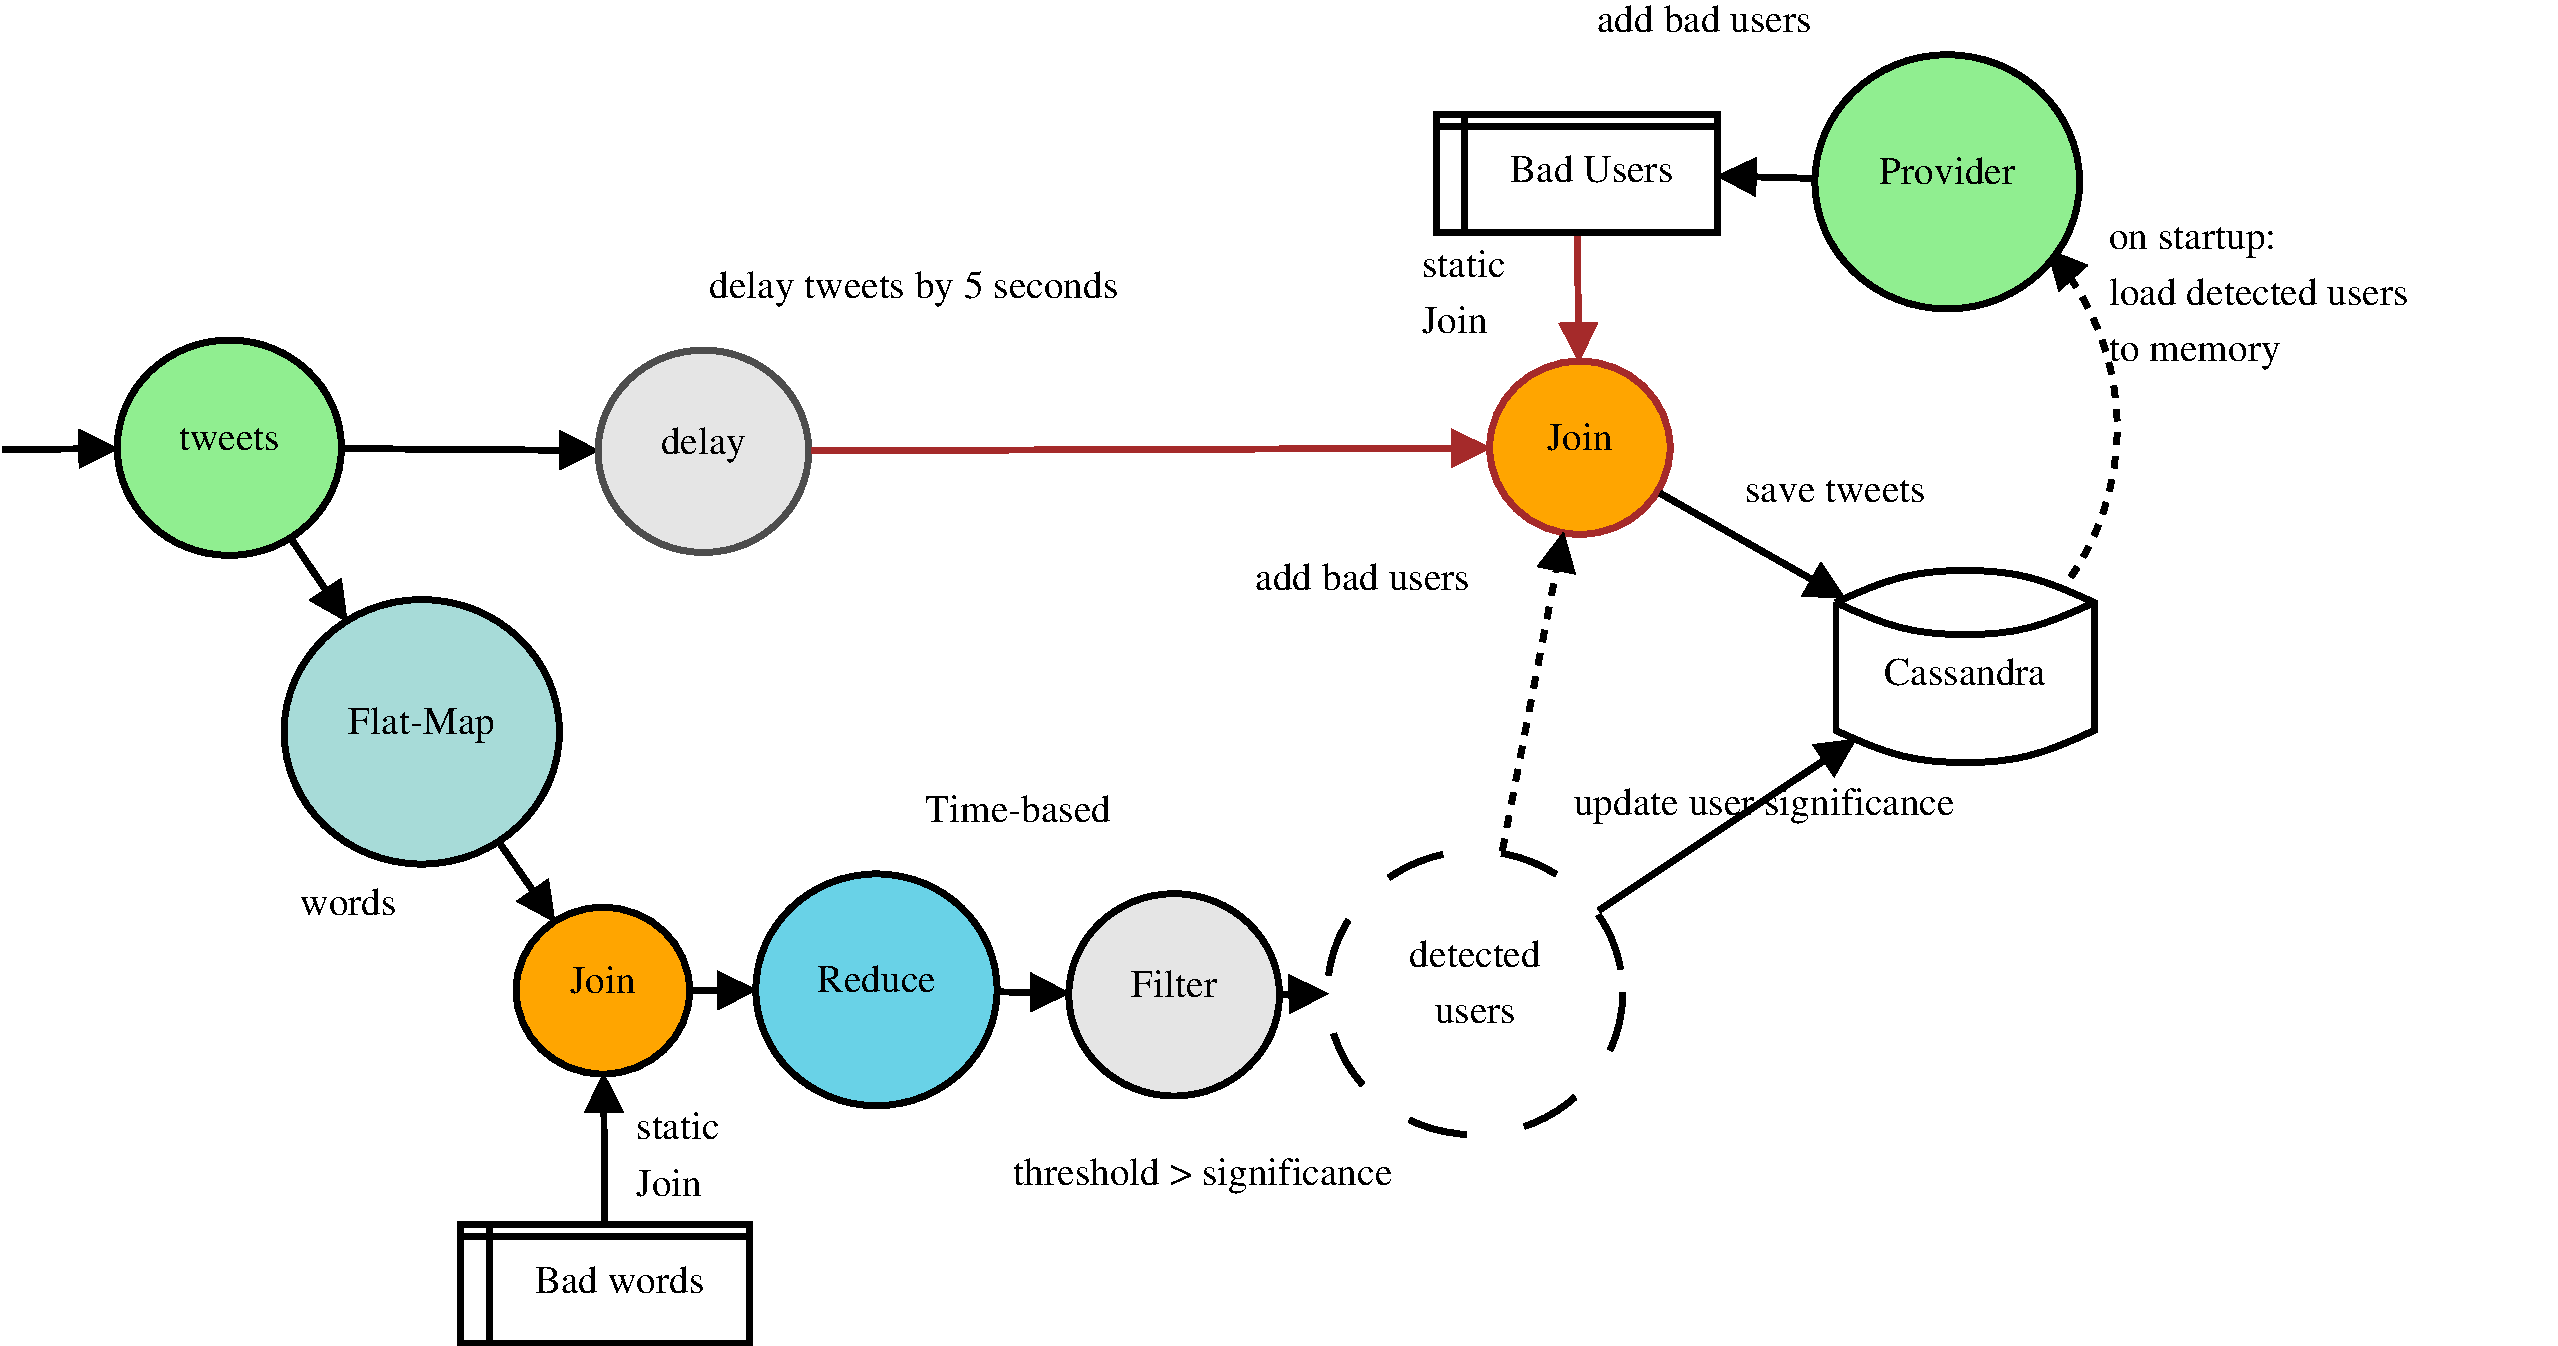
\includegraphics[width=0.55\textwidth]{images/AnalyzeTweetsTopology-eps-converted-to.pdf}
  \caption{This figure shows operators used in the topology and how they are related to each other. Operators are depicted as filled circles, in-memory storage is depicted as rectangles and dotted circles describe outputs within an operator for clarification.}
\end{figure}

\subsection{Topology}

The following section describe the topology used to the project use-case. The topology is divided two different streams orginated at the twitter stream source. The upper stream hold the tweets inside the topology until the second stream has analyzed the tweets and detected significanct users and inform the upper stream if it should skip or store tweets.

\subsubsection{Stream 1: Analyze Tweets}
\begin{description}
  \item[flatmap] \hfill \\
      Splits a whole tweet into single words and emit these words
      \newline output: \texttt{[Word,TweetId,User]}
  
  \item[join] \hfill \\
      Given is list of bad words. These bad words are joined with each of the words and emited with a predefined bad-word significance.
      \newline output: \texttt{[BadWord,TweetId,User,significance]}
  \item[reduce] \hfill \\
      The reducer compute the total-significance for a tweet. Each Bolt has to group the incoming tuples by \newline \texttt{[TweetId,User]}. The total-significance is computed a multiplication of all bad word occurences in a tweet.
      \newline output: \texttt{[TweetId,User,total-significance]}
      
  \item[filter] \hfill \\
      This filter operator allows to filter tweets above a specific significance threshold. In this Use-Case we set this to 1 to process all bad-words from users. The result are new detected users which are forwarded to the join operator of Stream 1 holding the tweets.

  \item[detected users] \hfill \\
      This dottet bolt is only to show the result of the whole stream. Detected users are forwarded to the join operator of Stream 1 holding the tweets. This needs a distinct tuple processing of incoming tuples from different sources. 
      
\end{description}

\subsubsection{Stream 2: Hold tweets}
\begin{description}
  \item[delay] \hfill \\
      The stream is orginated the the tweet stream source depicted in figure as an green node. The delayed bolt only hold the tweets for a specific time inside the topology until the tweets has been analyzed. The output is the same as the input.

  \item[join] \hfill \\
	The join operator received delayed tweet which are join with an in-memory hashtable containing detected users.
\end{description}

\subsection{Cassandra sink}
The cassandra sink operator takes care storing incoming tuples into cassandra tables. The operator analyze the incoming tuples, create new data structures if not exists and store theses tuples. The cassandra sink operator supports two different modes
\begin{description}
  \item[non-counter mode] \hfill \\
	The cassandra operator receives a specific key list and field-list which are stored persistently 
  \item[counter-mode] \hfill \\
       The counter-mode allows to increment fields by a specifc value located by initial key-fields.
\end{description}


\subsection{Cassandra provider}

The cassandra provider is only used if the topology is shut down and restarts again. The total user-significance is stored in cassandra and is reloaded to keep this in-memory to allow real-time processing. As an initial processing the cassandra-provider read all detected users with its significance and forwarded to the join operator. 

\subsection{Cassandra schema}
As an persistent storage cassandra is used to store detected users with its significance and their tweets. The cassandra-operator supports two different modes how to store data into the database. The \keyword{no-counter} mode assigns a specific primary-key to the incoming tuples an puts into a table. The \keyword{counter} mode only allows the increment a specific coulmn field determined by a primary-key.  

\begin{description}
  \item[user\_significance] \textit{counter} \hfill \\
  This tables stores for each user its significance-level which is increased over time. This table contains two columns, the twitter \keyword{user} and its \keyword{significance}. This table is loaded into the topology after an crash or an cluster-restart happened.
  
  \item[user\_tweets] \textit{counter}  \hfill \\
  This table stores the tweets for each user. The primary-key is \keyword{user} and \keyword{tweet\_id} with fields \keyword{tweet}.
  
  \item[word\_count]  \textit{non-counter} \hfill \\
  This table counts word occurences of bad words resulting in an user-update. The table provide some overall statistics.
  
\end{description}
    